\documentclass[a4paper,10pt]{article}
\usepackage[utf8]{inputenc}
\usepackage{url}
\usepackage{amsmath}
\usepackage{graphicx}
\usepackage{datetime}
\newdate{date}{09}{03}{2017}
\date{\displaydate{date}}

%opening
\title{COMP417\\Quiz on GraphSLAM\\First Name:\\Last Name:\\Student ID:}
\begin{document}

\maketitle

\subsubsection*{Each of the following questions is worth 1 point}
1. Suppose the 1D random variable $x$ has variance $\sigma_x^2=10$. Then the random variable $z=2x+1$ has variance: $\textbf{40}$
\newline
\newline
2. Suppose the 1D random variable $x$ has mean $\mu_x=10$. Then the random variable $z=2x+1$ has mean: $\textbf{21}$
\newline
\newline
3. Suppose the 2D random variable $\textbf{x}$ has covariance matrix $\boldsymbol{\Sigma}_x$. Then the covariance matrix of the random variable $\textbf{z}=\textbf{A}\boldsymbol{x} + \textbf{b}$, where $\textbf{b}$ is a 
constant vector is: $\textbf{A}\boldsymbol{\Sigma}\textbf{A}^T$
\newline
\newline
4. Suppose the 2D random variable $\textbf{x}$ has mean $\boldsymbol{\mu}_x$. Then the mean of the random variable $\textbf{z}=\textbf{A}\boldsymbol{x} + \textbf{b}$, where $\textbf{b}$ is a 
constant vector is: $\textbf{A}\boldsymbol{\mu}_x+\textbf{b}$
\newline
\newline
5. Write down the terms of the GraphSLAM cost function $J(\textbf{x}_1, \textbf{x}_2, \textbf{x}_3, \textbf{m}_0, \textbf{m}_1)$ for the scenario shown in Figure 1:
\begin{figure}[h]
  \begin{center}
    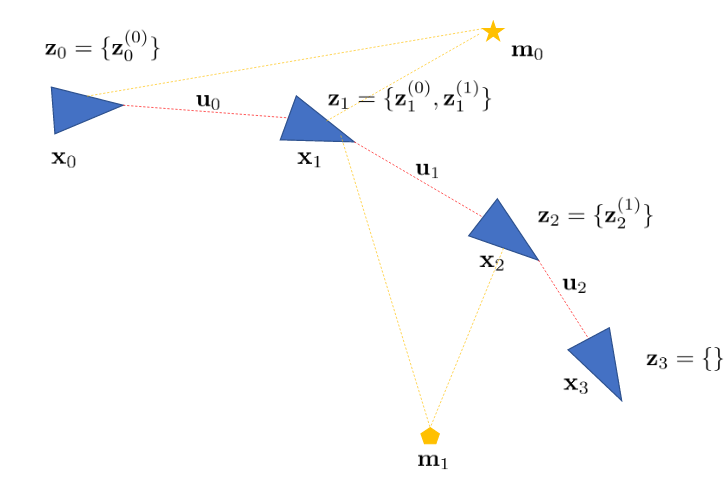
\includegraphics[width=0.7\textwidth]{quiz6fig}
  \end{center}
  \caption{State $\textbf{x}_0$ is known and fixed. The dynamics model is assumed to be $\textbf{x}_{t+1}=f(\textbf{x}_t, \textbf{u}_t) + \textbf{w}_t$ with $\textbf{w}_t \sim \mathcal{N}(\textbf{0}, \textbf{Q})$. 
  The observation model is assumed to be $\textbf{z}_t^{(k)}=h(\textbf{x}_t, \textbf{m}_k)+\textbf{n}_t$ where $\textbf{n}_t \sim \mathcal{N}(\textbf{0}, \textbf{R})$.}
\end{figure}
\newline
\newline
\begin{eqnarray}
   J(\textbf{x}_1, \textbf{x}_2, \textbf{x}_3, \textbf{m}_0, \textbf{m}_1) & = & ||\textbf{x}_{1} - f(\textbf{x}_0, \textbf{u}_0)||^2_{\textbf{Q}} +\nonumber \\
                                                                   {} &  & ||\textbf{x}_{2}-f(\textbf{x}_1, \textbf{u}_1) ||^2_{\textbf{Q}} +\nonumber \\
                                                                   {} &  & ||\textbf{x}_{3}-f(\textbf{x}_2, \textbf{u}_2) ||^2_{\textbf{Q}} +\nonumber \\
                                                                   {} &  & || \textbf{z}_0^{(0)} - h(\textbf{x}_0, \textbf{m}_0) ||^2_{\textbf{R}} +\nonumber \\
                                                                   {} &  & || \textbf{z}_1^{(0)} - h(\textbf{x}_1, \textbf{m}_0) ||^2_{\textbf{R}} +\nonumber \\
                                                                   {} &  & || \textbf{z}_1^{(1)} - h(\textbf{x}_1, \textbf{m}_1) ||^2_{\textbf{R}} +\nonumber \\
                                                                   {} &  & || \textbf{z}_2^{(1)} - h(\textbf{x}_2, \textbf{m}_1) ||^2_{\textbf{R}} \nonumber                                                                 
\end{eqnarray}
\newline
\newline
\newline
\newline
\newline
\newline
\newline
\newline
\newline
\newline
\newline
\newline
\newline
\newline
\newline
\newline
\newline
\newline
\newline




\end{document}
